% Options for packages loaded elsewhere
\PassOptionsToPackage{unicode}{hyperref}
\PassOptionsToPackage{hyphens}{url}
%
\documentclass[
]{article}
\usepackage{lmodern}
\usepackage{amssymb,amsmath}
\usepackage{ifxetex,ifluatex}
\ifnum 0\ifxetex 1\fi\ifluatex 1\fi=0 % if pdftex
  \usepackage[T1]{fontenc}
  \usepackage[utf8]{inputenc}
  \usepackage{textcomp} % provide euro and other symbols
\else % if luatex or xetex
  \usepackage{unicode-math}
  \defaultfontfeatures{Scale=MatchLowercase}
  \defaultfontfeatures[\rmfamily]{Ligatures=TeX,Scale=1}
\fi
% Use upquote if available, for straight quotes in verbatim environments
\IfFileExists{upquote.sty}{\usepackage{upquote}}{}
\IfFileExists{microtype.sty}{% use microtype if available
  \usepackage[]{microtype}
  \UseMicrotypeSet[protrusion]{basicmath} % disable protrusion for tt fonts
}{}
\makeatletter
\@ifundefined{KOMAClassName}{% if non-KOMA class
  \IfFileExists{parskip.sty}{%
    \usepackage{parskip}
  }{% else
    \setlength{\parindent}{0pt}
    \setlength{\parskip}{6pt plus 2pt minus 1pt}}
}{% if KOMA class
  \KOMAoptions{parskip=half}}
\makeatother
\usepackage{xcolor}
\IfFileExists{xurl.sty}{\usepackage{xurl}}{} % add URL line breaks if available
\IfFileExists{bookmark.sty}{\usepackage{bookmark}}{\usepackage{hyperref}}
\hypersetup{
  pdftitle={Seminar 1},
  pdfauthor={Eric},
  hidelinks,
  pdfcreator={LaTeX via pandoc}}
\urlstyle{same} % disable monospaced font for URLs
\usepackage[margin=1in]{geometry}
\usepackage{color}
\usepackage{fancyvrb}
\newcommand{\VerbBar}{|}
\newcommand{\VERB}{\Verb[commandchars=\\\{\}]}
\DefineVerbatimEnvironment{Highlighting}{Verbatim}{commandchars=\\\{\}}
% Add ',fontsize=\small' for more characters per line
\usepackage{framed}
\definecolor{shadecolor}{RGB}{248,248,248}
\newenvironment{Shaded}{\begin{snugshade}}{\end{snugshade}}
\newcommand{\AlertTok}[1]{\textcolor[rgb]{0.94,0.16,0.16}{#1}}
\newcommand{\AnnotationTok}[1]{\textcolor[rgb]{0.56,0.35,0.01}{\textbf{\textit{#1}}}}
\newcommand{\AttributeTok}[1]{\textcolor[rgb]{0.77,0.63,0.00}{#1}}
\newcommand{\BaseNTok}[1]{\textcolor[rgb]{0.00,0.00,0.81}{#1}}
\newcommand{\BuiltInTok}[1]{#1}
\newcommand{\CharTok}[1]{\textcolor[rgb]{0.31,0.60,0.02}{#1}}
\newcommand{\CommentTok}[1]{\textcolor[rgb]{0.56,0.35,0.01}{\textit{#1}}}
\newcommand{\CommentVarTok}[1]{\textcolor[rgb]{0.56,0.35,0.01}{\textbf{\textit{#1}}}}
\newcommand{\ConstantTok}[1]{\textcolor[rgb]{0.00,0.00,0.00}{#1}}
\newcommand{\ControlFlowTok}[1]{\textcolor[rgb]{0.13,0.29,0.53}{\textbf{#1}}}
\newcommand{\DataTypeTok}[1]{\textcolor[rgb]{0.13,0.29,0.53}{#1}}
\newcommand{\DecValTok}[1]{\textcolor[rgb]{0.00,0.00,0.81}{#1}}
\newcommand{\DocumentationTok}[1]{\textcolor[rgb]{0.56,0.35,0.01}{\textbf{\textit{#1}}}}
\newcommand{\ErrorTok}[1]{\textcolor[rgb]{0.64,0.00,0.00}{\textbf{#1}}}
\newcommand{\ExtensionTok}[1]{#1}
\newcommand{\FloatTok}[1]{\textcolor[rgb]{0.00,0.00,0.81}{#1}}
\newcommand{\FunctionTok}[1]{\textcolor[rgb]{0.00,0.00,0.00}{#1}}
\newcommand{\ImportTok}[1]{#1}
\newcommand{\InformationTok}[1]{\textcolor[rgb]{0.56,0.35,0.01}{\textbf{\textit{#1}}}}
\newcommand{\KeywordTok}[1]{\textcolor[rgb]{0.13,0.29,0.53}{\textbf{#1}}}
\newcommand{\NormalTok}[1]{#1}
\newcommand{\OperatorTok}[1]{\textcolor[rgb]{0.81,0.36,0.00}{\textbf{#1}}}
\newcommand{\OtherTok}[1]{\textcolor[rgb]{0.56,0.35,0.01}{#1}}
\newcommand{\PreprocessorTok}[1]{\textcolor[rgb]{0.56,0.35,0.01}{\textit{#1}}}
\newcommand{\RegionMarkerTok}[1]{#1}
\newcommand{\SpecialCharTok}[1]{\textcolor[rgb]{0.00,0.00,0.00}{#1}}
\newcommand{\SpecialStringTok}[1]{\textcolor[rgb]{0.31,0.60,0.02}{#1}}
\newcommand{\StringTok}[1]{\textcolor[rgb]{0.31,0.60,0.02}{#1}}
\newcommand{\VariableTok}[1]{\textcolor[rgb]{0.00,0.00,0.00}{#1}}
\newcommand{\VerbatimStringTok}[1]{\textcolor[rgb]{0.31,0.60,0.02}{#1}}
\newcommand{\WarningTok}[1]{\textcolor[rgb]{0.56,0.35,0.01}{\textbf{\textit{#1}}}}
\usepackage{graphicx,grffile}
\makeatletter
\def\maxwidth{\ifdim\Gin@nat@width>\linewidth\linewidth\else\Gin@nat@width\fi}
\def\maxheight{\ifdim\Gin@nat@height>\textheight\textheight\else\Gin@nat@height\fi}
\makeatother
% Scale images if necessary, so that they will not overflow the page
% margins by default, and it is still possible to overwrite the defaults
% using explicit options in \includegraphics[width, height, ...]{}
\setkeys{Gin}{width=\maxwidth,height=\maxheight,keepaspectratio}
% Set default figure placement to htbp
\makeatletter
\def\fps@figure{htbp}
\makeatother
\setlength{\emergencystretch}{3em} % prevent overfull lines
\providecommand{\tightlist}{%
  \setlength{\itemsep}{0pt}\setlength{\parskip}{0pt}}
\setcounter{secnumdepth}{-\maxdimen} % remove section numbering

\title{Seminar 1}
\author{Eric}
\date{18 1 2021}

\begin{document}
\maketitle

\hypertarget{velkommen-til-fuxf8rste-seminar}{%
\section{Velkommen til første
seminar!}\label{velkommen-til-fuxf8rste-seminar}}


\includegraphics{Bilder/Lovememe.png}

Gjennom 6 seminarganger skal vi nå gå igjennom alt fra hva R er og
hvordan det fungerer, til å kjøre våre helt egne regresjonsanalyser og
holde på med \emph{egen statistikk.} Jeg gleder meg! Før hvert seminar
kommer jeg til å legge ut et dokument som dette. Dette har jeg faktisk
laget i R! Her vil dere se at jeg har noe tekst (og memes, dere må like
memes), og noe kode. Dokumentet er det jeg har planlagt at vi skal gå
igjennom på seminaret, men det kan godt hende at vi gjør noe mindre der.
Etter det siste kommer det til å være en kort prøve. Om dere har noen
spørsmål må dere bare sende en melding! Det kan dere både gjøre på
e-post
(\href{mailto:egnilsen@student.sv.uio.no}{\nolinkurl{egnilsen@student.sv.uio.no}}),
og på Canvas!

\begin{Shaded}
\begin{Highlighting}[]
\CommentTok{#Kode vil dere se har en egen grå bakgrunn. Alt som er skrevet her kan dere kopiere inn på deres egen pc,}
\CommentTok{#og kjøre for å se hva som skjer. Når jeg har # foran betyr det at jeg skriver en kommentar. }
\CommentTok{#Dette kan vi gjøre i scriptene våre for å forklare hva som skjer, uten at R prøver å kjøre det som}
\CommentTok{#vanlig kode og derfor gir en feilmelding. }
\CommentTok{#Hvis jeg kjører kode her, vil dere se resultatene som vanlig tekst under. Vi kan jo gjøre et lite forsøk}
\CommentTok{# med noe enkel matte! For å kjøre koden setter dere musen ved siden av, og trykker ctrl+enter. }
\DecValTok{100}\OperatorTok{/}\DecValTok{2}\OperatorTok{+}\DecValTok{4}
\end{Highlighting}
\end{Shaded}

\begin{verbatim}
## [1] 54
\end{verbatim}

\hypertarget{r-rstudio-og-syntax-feil}{%
\section{R, RStudio, og Syntax-feil}\label{r-rstudio-og-syntax-feil}}


\includegraphics{Bilder/RStudio.png}

Før seminaret har dere lastet ned R, og RStudio. R er selve
programeringsspråket vi skriver i, og som gjør at vi kan skrive kode.
Når vi laster ned R laster vi egentlig ned et program som gjør at
datamaskingen vår kan forstå det vi skriver, og gjør det vi ønsker at
den gjør. Selve R-skriptet, eller koden om en vil, kunne vi egentlig
skrevet i word, eller notisblokk. RStudio, programmet vi kommer til å
bruke, er det som kalles et ``Integrated development environment''
(IDE), og brukes for å gjøre det lettere å skrive skriptet. Her har vi
f.eks. enkel tilgang til hjelpefiler, den markerer hva forskjellig kode
er ved hjelp av farger, og presenterer resultatene på en (vanligvis)
lettleselig måte.

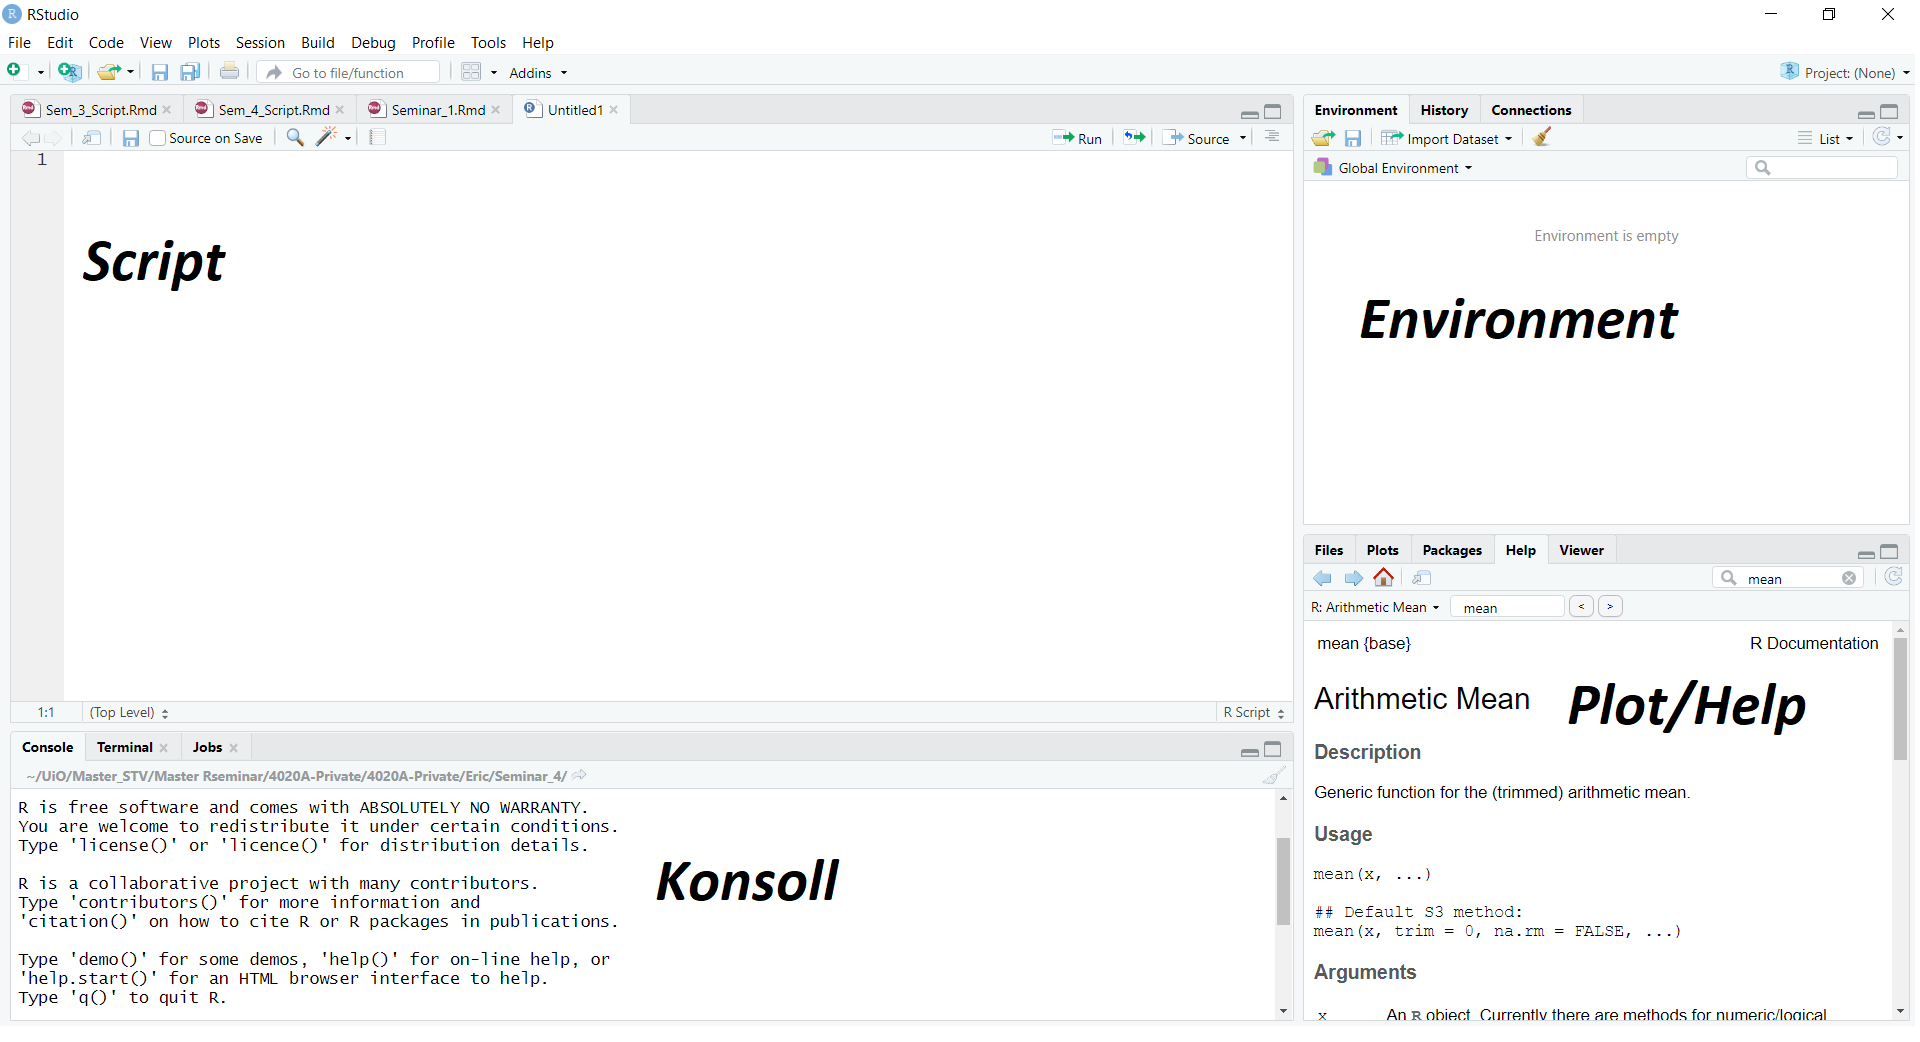
\includegraphics{Bilder/Panes.png}

Dere vil fort legge merke til at RStudio har flere vinduer. Øverst til
venstre (gitt standard konfigurasjonen, dere kan lett endre dette selv
om dere ønsker) finner dere selve skriptet. Det er her vi vil skrive
kode vi ønsker å lagre, og bruke videre. Under denne er det vi kaller
enn ``Konsoll'' eller ``intepreter'', når dere kjører kode vil dere se
at selve kodelinjen blir ``sendt'' ned dit, og det er der resultatet
vises. Vi kan også skrive kode direkte inn i konsollen, men da blir det
ikke lagret for senere bruk. Øverst til høyre har vi ``envoirement'',
her vises alle objekter som vi har laget i skriptet, hva dette er for
noe kommer vi tilbake til senere. Til slutt nederst til venstre vises en
del informasjon, hvor det er i hovedsak to faner vi kommer til å gjøre
bruk av. Den ene er ``Plots'' som veldig enkelt viser grafikk vi har
laget, f.eks. et stolpediagram, og den andre er hjelpefilene hvor en kan
slå opp hva forskjellige funksjoner gjør. Denne kan vi faktisk prøve ut
med en gang!

\begin{Shaded}
\begin{Highlighting}[]
\CommentTok{#Ofte når vi bruker R er vi usikre på hvordan forskjellige funksjoner fungerer. }
\CommentTok{#Da kan det være nyttig å lese hjelpefilene som forteller hva en funksjon gjør, og hvordan}
\CommentTok{#en skal bruke den. For å gjøre dette skriver du et spørsmålstegn før navnet på funksjonen. }
\CommentTok{#La oss prøve dette med "mean()" funksjonen, som logisk nok finner gjennomsnitt:}
\NormalTok{?mean}
\end{Highlighting}
\end{Shaded}

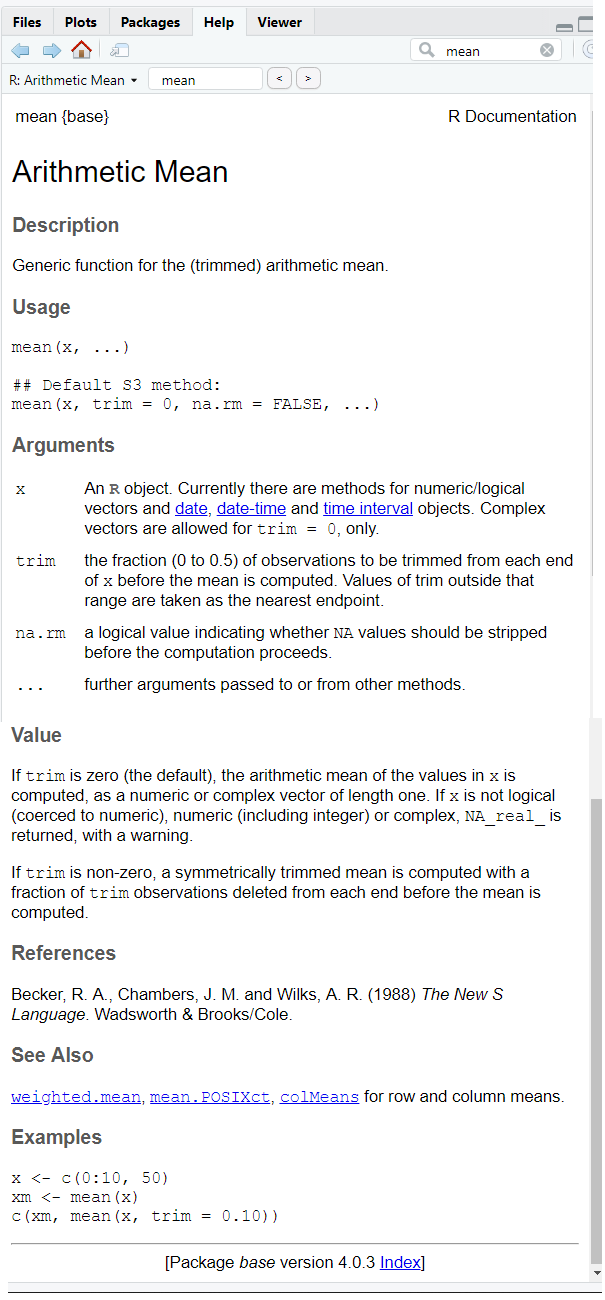
\includegraphics{Bilder/Help.png}

I hjelpefilen kan vi se at vi får en del informasjon om funksjonen, men
la oss først tenkte litt på hva en funksjon er. I R jobber vi som oftest
med forskjellige typer objekter. Vi skal straks komme tilbake til hva
objekter er, men la oss i første omgang tenke på en rekke tall. Si vi
har tallene fra 1-10. Hovedpoenget med R er at når vi har slike data,
ønsker vi å hente ut noe \emph{informasjon} fra dem. Dette kan f.eks.
være gjennomsnitt, standardavvvik ++. En funksjon er det vi bruker i R
for å gjøre noe med dataene, f.eks. å hente ut denne informasjonen. Alle
funksjoner har til felles at de tar noe data, f.eks. tall, og skaper et
resultat. I tilegg har noen argumenter som gjør at vi kan endre noe på
hvordan funksjonen lager resultatet. Leser vi hjelpefilen til ``mean''
ser vi at den øverst gir en beskrivelse, hvor det står at den returnerer
gjennomsnittet. Under der kommer argumentene den godtar, et objekt (x)
som inneholder tall, logiske verdier (kommer tilbake til hva det er),
ett argument for å trimme dataene, altså fjerne noe, og na.rm
argumentet. Det siste skal vi også komme tilbake til. Under Value får vi
en beskrivelse av hva som er returnert, før til slutt et eksempel av
hvordan den brukes i bunn.

Hjelpefilene er en flott måte å finne ut hva en funksjon gjør, og
hvordan vi kan bruke den. Samtidig kan den ofte være litt kronglete å
lese, men da hjelper det ofte å se på eksemplene som alltid er i bunn av
teksten. Skulle det fortsatt være vanskelig er det viktig å huske at det
finnes et stort miljø rundt R, og ofte er det mange som har opplevd
samme problem som deg! Litt kjapp googling, og et søk på
\url{https://stackoverflow.com/} vil fort gi gode svar!


\includegraphics{Bilder/Search.png}

\hypertarget{prosjekter-og-mapper}{%
\subsection{Prosjekter og mapper}\label{prosjekter-og-mapper}}

\begin{itemize}
\tightlist
\item
  Prosjekter hva/hvordan/hvorfor
\item
  Mappestruktur, keep it clean and simple
\end{itemize}

\hypertarget{syntax-feil}{%
\subsection{Syntax-feil}\label{syntax-feil}}

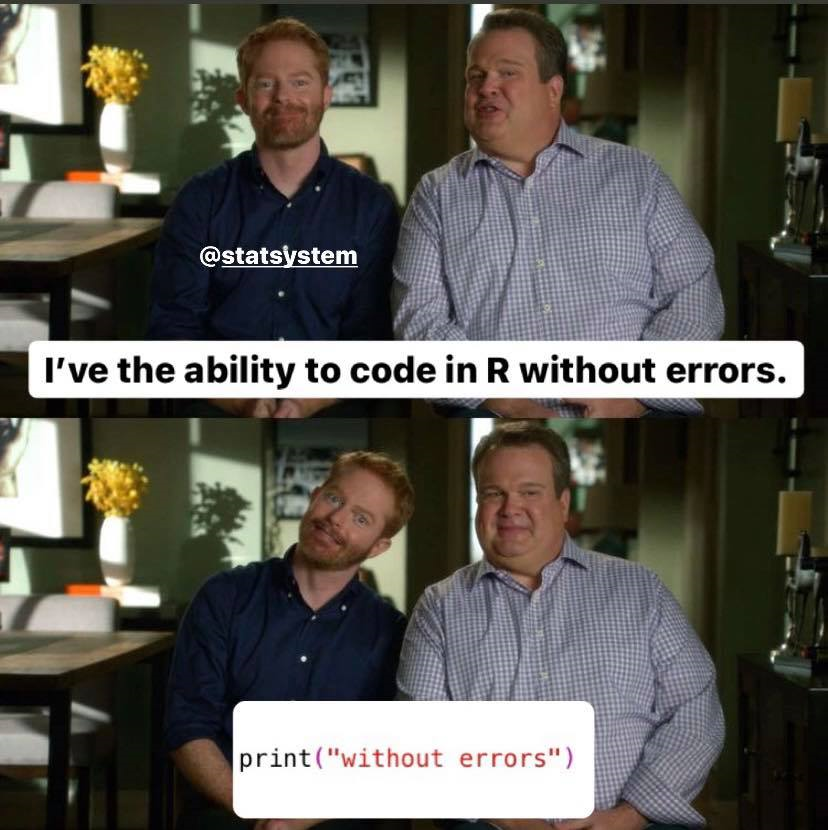
\includegraphics{Bilder/Error.png}

Når vi går igjennom kode vil vi fort få en del feil. Det er helt vanlig,
og noe som er helt uungåelig! Dere vil nok fort merke at jeg gjør en hel
del feil når jeg skal vise dere i seminaret. En type feil kan likevell
være godt å merke seg med en gang, mest fordi jeg gjør den hver gang jeg
skal skrive noe kode. ``Syntax-feil'' er skrivefeil vi gjør når vi
skriver kode. F.eks. kan det være å skrive men() istedenfor mean(),
glemme å lukke en parantes sånn at vi skriver mean( . Noe av det fine
med RStudio er at den markere sånne feil for oss!

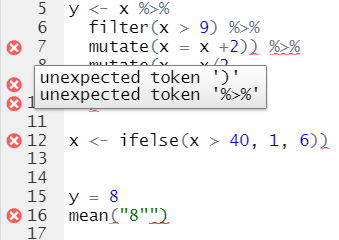
\includegraphics{Bilder/TulleFeil.png}

Her har jeg skrevet noe tullekode for å vise ossen dette funker. Som
dere kan se på siden får jeg flere røde kryss ved siden av
linjenummerene. Dette er steder hvor RStudio mener jeg har gjort feil,
og holder jeg musen over dem får jeg opp hva som er feilen. ``Unexpected
token `)'\,'' betyr at RStudio mener det er en parantes der som ikke
skulle vært der. I tilegg er det røde streker under de delene av koden
som RStudio mener er feil. Jeg vil hevde, hvertfall etter min egen
erfaring, at 90 \% av feilene vi gjør i R er enkle
skrivefeil/syntax-feil som dette. Derfor er det veldig nyttig at RStudio
viser det på denne måten!


\includegraphics{Bilder/Coding.jpg}

\hypertarget{objekter-funksjoner-og-klasser}{%
\section{Objekter, funksjoner, og
klasser}\label{objekter-funksjoner-og-klasser}}

Vi har allerede sett på litt enkel kode, men framover skal vi gått litt
dypere inn i hvordan kode faktisk fungerer. Logisk nok er koding en måte
fortelle pc'n hva vi vil den skal gjøre gjennom tekst. Sånn sett er det
nærmest det samme som når du klikker på noe, bare at dette er noe mer
effektivt. Når vi skriver kode må vi vite hva vi skal skrive for at pc'n
skal forstå det. All den tid det ikke finnes noen enorm ordbok som
forteller alt vi kan skrive i R er dette noe vi må lære oss, og kanskje
pugge, eller bare søkte etter når vi trenger det. Den vanligste måten å
lære nye koder på er å google etter spesifikke ting du ønsker å gjøre.

Det første vi skal se på nå er objekter. Objekter er i alle ``ting'' i R
som kan inneholde noe annet. Vi skal i hovedsak forholde oss til to
typer objekter vektorer, og funksjoner. Hva disse er nok lettere å vise
ved eksempel:

\begin{Shaded}
\begin{Highlighting}[]
\CommentTok{#Her ønsker jeg å lage et objekt. I første omgang kan vi prøve å lage en vektor. Dette er et objekt}
\CommentTok{#som inneholder flere elementer, f.eks. tall av samme klasse. La oss først prøve å lage en med ett}
\CommentTok{#tall. For å gjøre dette må vi først velge et navn, så bruke det som heter en "assigner", og så}
\CommentTok{#skrive hva den skal inneholde. Her lager jeg en vektor som heter "To" og som inneholder tallet 2. }
\NormalTok{To <-}\StringTok{ }\DecValTok{2}
\CommentTok{# <- er det som er assigneren. Den sier bare at det som kommer på venstresiden skal lagres med }
\CommentTok{#navnet som er på høyresiden. Om dere kjører koden (ctrl+enter med musen ved siden av, eller}
\CommentTok{#teksten markert) vil dere se i envoirnment at det kommer en linje hvor det står "To   2", dette}
\CommentTok{#betyr at vi har laget en variabel med navn To som inneholder verdien 2. }
\CommentTok{#Nå som vi har et objekt kan vi begynne å bruke det til noe. Først kan vi prøve å gjøre matte igjen:}
\DecValTok{2} \OperatorTok{+}\StringTok{ }\NormalTok{To }
\end{Highlighting}
\end{Shaded}

\begin{verbatim}
## [1] 4
\end{verbatim}

\begin{Shaded}
\begin{Highlighting}[]
\CommentTok{#Som dere ser kan jeg nå skrive 2 + To og få ut resultatet fire. Når vi nå skriver "To" vet R at vi}
\CommentTok{# *egentlig* mener tallet 2. For så enkle ting som dette er sikkert enklere å bare skrive 2, eller}
\CommentTok{#bare bruke en kalkulator for den saks skyld. Det fine med objekter er at de kan inneholde veldig mye}
\CommentTok{#informasjon! I første omgang kan vi prøve å lagre flere tall. Det er flere måter vi kan gjøre dette}
\CommentTok{#på, f.eks. kan vi skrive 1:10 for å få alle heltallene mellom 1 og 10, eller skrive c(1,22,5,2,1) for}
\CommentTok{#å lage en rekke tall. I det siste skiller jeg tallene med komma. Objektene kan hete hva du vil forøvrig. }
\NormalTok{Hva_Du_Vil <-}\StringTok{ }\DecValTok{1}\OperatorTok{:}\DecValTok{100}
\NormalTok{Forovrig <-}\StringTok{ }\KeywordTok{c}\NormalTok{(}\DecValTok{1}\NormalTok{,}\DecValTok{4}\NormalTok{,}\DecValTok{56}\NormalTok{,}\DecValTok{8}\NormalTok{,}\DecValTok{4}\NormalTok{,}\DecValTok{2}\NormalTok{,}\DecValTok{4}\NormalTok{)}
\CommentTok{#Eneste er at du ikke kan ha mellomrom i navnene eller tall som første tegn, og det er god kutyme å unnå}
\CommentTok{#æ/ø/å generelt i script.}
\CommentTok{#Nå som vi har et script med flere elementer kan vi prøve å kjøre noen funksjoner på dem}
\CommentTok{#Det kan nevnes at funksjoner faktisk er objekter de og, men det blir først innteresant når du holder}
\CommentTok{#på med litt mer avansert kode. La oss se om vi kan finne gjennomsnittet av disse vektorene. }
\KeywordTok{mean}\NormalTok{(Forovrig)}
\end{Highlighting}
\end{Shaded}

\begin{verbatim}
## [1] 11.28571
\end{verbatim}

\begin{Shaded}
\begin{Highlighting}[]
\KeywordTok{mean}\NormalTok{(Hva_Du_Vil)}
\end{Highlighting}
\end{Shaded}

\begin{verbatim}
## [1] 50.5
\end{verbatim}

Med mean funksjonen her ser vi at vi får gjennomsnittet for hele
vektoren. Som oftest er det det vi ønsker, men hva hvis vi kun ønsket
gjennomsnittet av noen tall? Om dere ser tilbake til envoirenment vil
dere merke at etter navnet på vektoren står det først ``num'' og så
{[}1:7{]}. Den første teksen sier at dette er et numerisk objekt.
Klasser skal vi straks gå inn på. Det neste viser lengden på vektoren
vår. \emph{Forovrig} har sitt første tall i plassen 1, og siste i 7.
Altså er det 7 ellementer. Om vi ser på \emph{hva du vil} ser vi at det
står 1:100, og denne har altså 100 elementer. For å få tak i et
spesifikt element kan vi bruke disse klammeparantesene.

\begin{Shaded}
\begin{Highlighting}[]
\CommentTok{#La oss si at vi vil ha element nr. 5 i vektoren Forovrig.}
\NormalTok{Forovrig[}\DecValTok{5}\NormalTok{] }\CommentTok{#Når vi kjører denne ser vi at vi får ut tallet 5,}
\end{Highlighting}
\end{Shaded}

\begin{verbatim}
## [1] 4
\end{verbatim}

\begin{Shaded}
\begin{Highlighting}[]
            \CommentTok{#og dette kan vi jo også sjekke i envorement for å se at stemmer. }

\CommentTok{#På samme måte som vi definerte en rekke tall istad, kan vi også bruke dette}
\CommentTok{#for å få ut en rekke elementer. }

\NormalTok{Forovrig[}\DecValTok{3}\OperatorTok{:}\DecValTok{6}\NormalTok{]}
\end{Highlighting}
\end{Shaded}

\begin{verbatim}
## [1] 56  8  4  2
\end{verbatim}

\begin{Shaded}
\begin{Highlighting}[]
\NormalTok{Forovrig[}\KeywordTok{c}\NormalTok{(}\DecValTok{3}\NormalTok{,}\DecValTok{5}\NormalTok{,}\DecValTok{3}\NormalTok{,}\DecValTok{6}\NormalTok{)]}
\end{Highlighting}
\end{Shaded}

\begin{verbatim}
## [1] 56  4 56  2
\end{verbatim}

\begin{Shaded}
\begin{Highlighting}[]
\CommentTok{#Her kan vi også finne gjennomsnittet av kun disse tallene}
\KeywordTok{mean}\NormalTok{(Forovrig[}\KeywordTok{c}\NormalTok{(}\DecValTok{3}\NormalTok{,}\DecValTok{5}\NormalTok{,}\DecValTok{3}\NormalTok{,}\DecValTok{6}\NormalTok{)])}
\end{Highlighting}
\end{Shaded}

\begin{verbatim}
## [1] 29.5
\end{verbatim}

\begin{Shaded}
\begin{Highlighting}[]
\CommentTok{#Eller bruke disse som en ny vekter}
\NormalTok{Ny_Vektor <-}\StringTok{ }\NormalTok{Forovrig[}\KeywordTok{c}\NormalTok{(}\DecValTok{3}\NormalTok{,}\DecValTok{5}\NormalTok{,}\DecValTok{3}\NormalTok{,}\DecValTok{6}\NormalTok{)]}
\end{Highlighting}
\end{Shaded}

\hypertarget{klasser}{%
\subsection{Klasser}\label{klasser}}

Så langt har vi kun jobbet med tallverdier. Ofte har vi variabler som
ikke er tall, men f.eks. tekst eller ordinalverdier. I R vil vi også se
at visse funksjoner krever at dataene er i visse klasser. Hovedklassene
vi kommer til å bruke er; numeric, character, logical, og factor.
Numeric er tall (logisk nok). De fleste mattefunksjoner krever at
dataene er numeric.

\begin{Shaded}
\begin{Highlighting}[]
\CommentTok{#For å sjekke om noe er numeric kan vi bruke funksjonen is.numeric()}

\KeywordTok{is.numeric}\NormalTok{(Hva_Du_Vil)}
\end{Highlighting}
\end{Shaded}

\begin{verbatim}
## [1] TRUE
\end{verbatim}

\begin{Shaded}
\begin{Highlighting}[]
\CommentTok{#Her ser vi at vi får opp "TRUE" som betyr at Hva_Du_Vil er et numerisk objekt}
\end{Highlighting}
\end{Shaded}

Dere vil noen ganger se at det skilles mellom ``numeric'' og
``integer''. Forskjellen er at integer kun kan inneholde heltall, mens
numeric kan ha desimaler. Dette er noe som henger igjen fra gammelt av,
og er svært sjeldent interessant for vår del.

Når vi vil skrive tekst bruker vi klassen ``character''. En tekststring
må alltid ha "" rundt seg, men ellers definerer vi den som vanlig.

\begin{Shaded}
\begin{Highlighting}[]
\NormalTok{Tekst <-}\StringTok{ "Hei, jeg elsker R! <3"}
\CommentTok{#Denne klassen kan inneholde tekst, men vil f.eks. ikke kunne brukes til matte. }
\KeywordTok{mean}\NormalTok{(Tekst)}
\end{Highlighting}
\end{Shaded}

\begin{verbatim}
## Warning in mean.default(Tekst): argument is not numeric or logical: returning NA
\end{verbatim}

\begin{verbatim}
## [1] NA
\end{verbatim}

\begin{Shaded}
\begin{Highlighting}[]
\CommentTok{#Her ser dere at vi får en feilmelding, som sier at argumentet ikke er}
\CommentTok{#numerisk eller logisk. Funksjonen gir oss derfor resultatet NA, som}
\CommentTok{#betyr missing, altså at det ikke eksisterer et resultat. }

\CommentTok{#Vi kan også kreve at et objekt skal ha en viss klasse. Det gjør vi med}
\CommentTok{#as. "klassenavn". Det kan føre til noen uforventede resultater. Si hvis gjør}
\CommentTok{#Forovrig om til character. }
\NormalTok{Forovrig <-}\StringTok{ }\KeywordTok{as.character}\NormalTok{(Forovrig)}
\KeywordTok{mean}\NormalTok{(Forovrig)}
\end{Highlighting}
\end{Shaded}

\begin{verbatim}
## Warning in mean.default(Forovrig): argument is not numeric or logical: returning
## NA
\end{verbatim}

\begin{verbatim}
## [1] NA
\end{verbatim}

Grunnen til at vi får en feilmelding her er fordi vi ikke kan ta
gjenomsnittet av tekst. Om dere ser i envoirement står det også nå at
Forovrig er chr (charater) og det "" rundt alle tegnene.

Den siste klassen vi kommer til å bruke ofte (men det finnes flere) er
``factor.'' Faktor er en variabel som kan ha flere forhåndsdefinerte
nivåer, og brukes ofte når vi skal kjøre statistiske modeller. En lett
måte å forstå factorer på er å tenke på dem som ordinale variabler, hvor
vi kan vite rekkefølgen på nivåene men ikke avstanden, f.eks.
Barneskole, Ungdomskole, vgs.

\begin{Shaded}
\begin{Highlighting}[]
\NormalTok{Skolenivaer <-}\StringTok{ }\KeywordTok{factor}\NormalTok{(}\KeywordTok{c}\NormalTok{(}\StringTok{"Barneskole"}\NormalTok{, }\StringTok{"Ungdomskole"}\NormalTok{, }\StringTok{"Videregaende"}\NormalTok{, }\StringTok{"Videregaende"}\NormalTok{, }\StringTok{"Ungdomskole"}\NormalTok{),}
\DataTypeTok{levels =} \KeywordTok{c}\NormalTok{(}\StringTok{"Barneskole"}\NormalTok{, }\StringTok{"Ungdomskole"}\NormalTok{, }\StringTok{"Videregaende"}\NormalTok{))}

\CommentTok{#Her kan vi se at vi først definerer de forskjellige verdiene som er i variabelen}
\CommentTok{#Så skriver vi hvilke nivåer den kan ha, i den rekkefølgen vi ønsker dem}
\CommentTok{#Om vi ikke hadde definert nivåene ville R gjort det automatisk i alfabetisk}
\CommentTok{#rekkefølge, som oftest går det greit men noen ganger ønsker vi det annerledes}
\CommentTok{#Nå kan vi først se på hva som er i variabelen}
\NormalTok{Skolenivaer }\CommentTok{#Kjører vi bare denne ser vi alle verdiene}
\end{Highlighting}
\end{Shaded}

\begin{verbatim}
## [1] Barneskole   Ungdomskole  Videregaende Videregaende Ungdomskole 
## Levels: Barneskole Ungdomskole Videregaende
\end{verbatim}

\begin{Shaded}
\begin{Highlighting}[]
\CommentTok{#Vi kan også se hvilke nivåer som er i variabelen}
\KeywordTok{levels}\NormalTok{(Skolenivaer) }\CommentTok{#Og får ut de tre nivåene}
\end{Highlighting}
\end{Shaded}

\begin{verbatim}
## [1] "Barneskole"   "Ungdomskole"  "Videregaende"
\end{verbatim}

I toppen her sa jeg at en vektor var et objekt som inneholdt elementer
av \emph{samme} klasse. Så langt har vi også holdt oss til det gjennom å
kune lage objekter med tekst eller tall. Hva skjer da om vi prøver å
blande?

\begin{Shaded}
\begin{Highlighting}[]
\CommentTok{#Nå kan vi lage et objekt som inneholder både tekst og tall:}
\NormalTok{TekstTall <-}\StringTok{ }\KeywordTok{c}\NormalTok{(}\DecValTok{1}\NormalTok{,}\DecValTok{4}\NormalTok{,}\DecValTok{0}\NormalTok{,}\DecValTok{4}\NormalTok{, }\StringTok{"Bamse"}\NormalTok{, }\StringTok{"R"}\NormalTok{, }\StringTok{"R Seminarer er de BESTE seminarer"}\NormalTok{, }\DecValTok{42}\NormalTok{, }\StringTok{"the answer"}\NormalTok{)}
\CommentTok{#Nå kan vi bruke funksjonen "class()" for å se hvilken klasse dette nye objektet har}
\KeywordTok{class}\NormalTok{(TekstTall)}
\end{Highlighting}
\end{Shaded}

\begin{verbatim}
## [1] "character"
\end{verbatim}

Som vi kan se er her klassen blitt character, også for tallene! Det er
fordi at hvis vi definerer en vektor som har flere klasser, blir det
slått sammen til den klassen som har minst informasjon. Dette kalles
``implicit coercion'', og rekkefølgen går: logical -\textgreater{}
integer -\textgreater{} numeric -\textgreater{} complex -\textgreater{}
character.

\hypertarget{dataframes}{%
\section{Dataframes}\label{dataframes}}

Noen ganger har vi lyst til å slå sammen data som er av forskjellige
typer. F.eks. kan det være at vi har data om alder, navn, fylke etc. og
vil ha dette som et objekt. For å gjøre dette bruker vi data.frames. En
dataframe består av flere kolloner, hvor hver kollone er en vektor.
Disse kan ha forskjellige typer, med f.eks. en character vektor, og ett
tall. Videre vil hver rad være en enhet. Dette kan f.eks. være en
person. Data.frames er ofte noe en laster ned når en skal ha data,
f.eks. fra en survey, men vi kan også lage dem selv. En viktig regel for
dataframes er at alle vektorene må ha lik lengde. Om vi dermed mangler
noen observasjoner må vi finne en måte å ``fylle'' disse tomme cellene.
Det gjør vi med NA.

\begin{Shaded}
\begin{Highlighting}[]
\NormalTok{Navn <-}\StringTok{ }\KeywordTok{c}\NormalTok{(}\StringTok{"Arne"}\NormalTok{, }\StringTok{"Geir"}\NormalTok{, }\StringTok{"Hans"}\NormalTok{, }\StringTok{"Kleopatra"}\NormalTok{, }\StringTok{"Mari"}\NormalTok{, }\StringTok{"Gunnar"}\NormalTok{, }\StringTok{"Kalle"}\NormalTok{)}
\NormalTok{Alder <-}\StringTok{ }\KeywordTok{c}\NormalTok{(}\DecValTok{60}\NormalTok{, }\DecValTok{45}\NormalTok{, }\DecValTok{19}\NormalTok{, }\DecValTok{19}\NormalTok{, }\OtherTok{NA}\NormalTok{, }\DecValTok{87}\NormalTok{, }\DecValTok{92}\NormalTok{)}
\NormalTok{Fylke <-}\StringTok{ }\KeywordTok{c}\NormalTok{(}\StringTok{"Telemark"}\NormalTok{, }\StringTok{"Finnmark"}\NormalTok{, }\StringTok{"Buskerud"}\NormalTok{, }\OtherTok{NA}\NormalTok{, }\StringTok{"Hordaland"}\NormalTok{, }\StringTok{"Vestfold"}\NormalTok{, }\StringTok{"Trøndelag"}\NormalTok{ )}
\NormalTok{By <-}\StringTok{ }\KeywordTok{c}\NormalTok{(}\StringTok{"Skien"}\NormalTok{, }\StringTok{"karasjok"}\NormalTok{, }\StringTok{"Kongsberg"}\NormalTok{, }\OtherTok{NA}\NormalTok{, }\StringTok{"Dale"}\NormalTok{, }\StringTok{"Stokke"}\NormalTok{, }\StringTok{"Trondhjem"}\NormalTok{)}
\CommentTok{#Her lager jeg først et sett med vektorer, med litt forskjellig informasjon.}
\CommentTok{#Dere kan se i envoirnment at alle har en lengde på 7. Dette kan vi også sjekke med}
\CommentTok{#length() funksjonen. }
\KeywordTok{length}\NormalTok{(Navn)}
\end{Highlighting}
\end{Shaded}

\begin{verbatim}
## [1] 7
\end{verbatim}

\begin{Shaded}
\begin{Highlighting}[]
\CommentTok{#For å lage en data.frame kan vi bruke funksjones as.data.frame()}

\NormalTok{Personer <-}\StringTok{ }\KeywordTok{data.frame}\NormalTok{(Navn, Alder, Fylke, By)}
\end{Highlighting}
\end{Shaded}

I environment vil dere nå se at det dukker opp en ny type verdi, under
``Data'' med navnet Personer. Når det står 7 obs (observasjoner) av 4
variabler betyr dette at vi har en dataframe med 7 rader og 4 kolloner.
Klikker dere på den vil dere se dette.

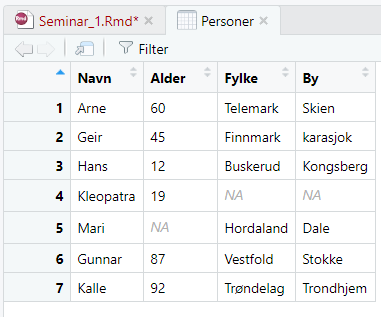
\includegraphics{Bilder/DF.png}

Første observasjonen her er rad 1, som er Arne på 60 år fra Skien i
Telemark (Norges beste by og fylke forøvrig.) Det viktigste med en
dataframe er at vi nå kan sette sammen flere typer informasjon om samme
enhet på en gang. Det er flere måter vi kan bruke dette på. La oss først
se på hvordan vi kan gjøre enkle analyser av en kollone.

\begin{Shaded}
\begin{Highlighting}[]
\CommentTok{#Før har vi kun skrevet navnet på vektoren. Nå som vi har det i en dataframe, må vi først}
\CommentTok{#velge denne, og så kolonnen. Det er to måter vi kan gjøre dette på:}
\NormalTok{Personer[}\DecValTok{2}\NormalTok{,}\DecValTok{1}\NormalTok{] }\CommentTok{#Med klammeparanteser kan vi velge rad og kolonne. Rad kommer først, og så kolonnen. }
\end{Highlighting}
\end{Shaded}

\begin{verbatim}
## [1] "Geir"
\end{verbatim}

\begin{Shaded}
\begin{Highlighting}[]
\NormalTok{Personer[,}\DecValTok{2}\NormalTok{] }\CommentTok{#Skriver vi en tom får vi alle kollonene/radene }
\end{Highlighting}
\end{Shaded}

\begin{verbatim}
## [1] 60 45 19 19 NA 87 92
\end{verbatim}

\begin{Shaded}
\begin{Highlighting}[]
\NormalTok{Personer[}\DecValTok{2}\NormalTok{,]}
\end{Highlighting}
\end{Shaded}

\begin{verbatim}
##   Navn Alder    Fylke       By
## 2 Geir    45 Finnmark karasjok
\end{verbatim}

\begin{Shaded}
\begin{Highlighting}[]
\CommentTok{#Noen ganger er det ønskelig å velge ut noen grupper i datasettet. }
\CommentTok{#Samtidig blir det fort vanskelig å huske tallet til plasseringen,}
\CommentTok{#neste gang skal vi derfor se på noen lettere måter å gjøre dette på. }

\CommentTok{#En mer vanlig måte å hente ut kolonner på er med '$'.}
\NormalTok{Personer}\OperatorTok{$}\NormalTok{Alder }\CommentTok{#Her skriver jeg først navnet på dataframen, og så variabelen}
\end{Highlighting}
\end{Shaded}

\begin{verbatim}
## [1] 60 45 19 19 NA 87 92
\end{verbatim}

\begin{Shaded}
\begin{Highlighting}[]
               \CommentTok{#Som dere ser får jeg ut verdien på alle aldrene}

\CommentTok{#Her kan vi bruke mattematiske formler på samme måte som istad.}
\CommentTok{#La oss prøve å få ut gjennomsnitt og alder på personene. }

\KeywordTok{mean}\NormalTok{(Personer}\OperatorTok{$}\NormalTok{Alder)}
\end{Highlighting}
\end{Shaded}

\begin{verbatim}
## [1] NA
\end{verbatim}

Hm. Her kan dere se at vi fikk NA til svar istedet for det
gjennomsnittet vi ønsket. NA betyr som sagt bare missing, altså at vi
ikke har informasjon om noe. For Mari i datasettet har vi ikke
informasjon om hvor gammel hun er. Når minst en av verdiene er NA vil
flere funksjoner også returnere NA. Dette fordi vi jo strengt tatt ikke
kan vite gjennomsnittet om vi ikke vet alle verdiene. For å få ut et
resultat må vi derfor fortelle R at vi ønsker å fjerne NA verdiene, og
heller få gjenomsnittet av de verdiene som er tilstede.

\begin{Shaded}
\begin{Highlighting}[]
\KeywordTok{mean}\NormalTok{(Personer}\OperatorTok{$}\NormalTok{Alder, }\DataTypeTok{na.rm =} \OtherTok{TRUE}\NormalTok{) }\CommentTok{#Her ser dere at vi får svaret 52.5 istedet.}
\end{Highlighting}
\end{Shaded}

\begin{verbatim}
## [1] 53.66667
\end{verbatim}

\begin{Shaded}
\begin{Highlighting}[]
                                   \CommentTok{#na.rm betyr NA remove, og når vi setter den til TRUE ber R}
                                   \CommentTok{#om å fjerne disse NA. }


\CommentTok{#Eller median for å finne median}
\KeywordTok{median}\NormalTok{(Personer}\OperatorTok{$}\NormalTok{Alder, }\DataTypeTok{na.rm =} \OtherTok{TRUE}\NormalTok{)}
\end{Highlighting}
\end{Shaded}

\begin{verbatim}
## [1] 52.5
\end{verbatim}

\begin{Shaded}
\begin{Highlighting}[]
\CommentTok{#En lettere måte å få ut alle disse på er ved å bruke summary() funksjonen.}
\CommentTok{#Da trenger vi heller ikke bruke na.rm, fordi den heller sier hvor mange NA }
\CommentTok{#det er i vektoren}

\KeywordTok{summary}\NormalTok{(Personer}\OperatorTok{$}\NormalTok{Alder)}
\end{Highlighting}
\end{Shaded}

\begin{verbatim}
##    Min. 1st Qu.  Median    Mean 3rd Qu.    Max.    NA's 
##   19.00   25.50   52.50   53.67   80.25   92.00       1
\end{verbatim}

\hypertarget{visualisering}{%
\section{Visualisering}\label{visualisering}}

Det siste vi skal på idag er en kort intro til hvordan vi kan
visualisere data. For å gjøre dette må vi først laste ned en pakke som
heter Tidyverse. Pakker er tilegg til R som gjør at du kan laste ned
flere funksjoner, og ofte gjør visse ting enklere. R som det kommer når
det lastes ned kalles ``base R.'' Om noe er vanskelig i base R, finnes
det høyst sansynelig en pakke som gjør det lettere! Tidyverse, som vi
vil bruke mye, er et sett med pakker som gjør databehandling mye, mye
enklere. For å bruke denne må vi først innstalere pakken. Om dere har
gjort dette på forhånd trenger dere ikke gjøre dette på nytt. Å
installere gjør vi kun en gang, og så evt. på nytt om det kommer en
oppdatering.

\begin{Shaded}
\begin{Highlighting}[]
\KeywordTok{install.packages}\NormalTok{(}\StringTok{"tidyverse"}\NormalTok{)}
\CommentTok{#For å innstalere bruker vi funksjonen install.packages, og skriver navnet på}
\CommentTok{#pakken i parantesene med hermetegn}
\end{Highlighting}
\end{Shaded}

Hver gang vi skal bruke pakken må vi fortelle R at vi skal bruke den.
Det må vi gjøre hver gang vi åpner R på nytt.

\begin{Shaded}
\begin{Highlighting}[]
\CommentTok{#For å gjøre dette bruker vi funksjonen library()}
\KeywordTok{library}\NormalTok{(}\StringTok{"tidyverse"}\NormalTok{)}
\end{Highlighting}
\end{Shaded}

\begin{verbatim}
## -- Attaching packages --------------------------------------- tidyverse 1.3.0 --
\end{verbatim}

\begin{verbatim}
## v ggplot2 3.3.2     v purrr   0.3.4
## v tibble  3.0.4     v dplyr   1.0.2
## v tidyr   1.1.2     v stringr 1.4.0
## v readr   1.4.0     v forcats 0.5.0
\end{verbatim}

\begin{verbatim}
## -- Conflicts ------------------------------------------ tidyverse_conflicts() --
## x dplyr::filter() masks stats::filter()
## x dplyr::lag()    masks stats::lag()
\end{verbatim}

Tidyverse skal vi bruke masse tid på nesten gang, men akkurat nå skal vi
se på en del av det som heter ggplot. GGplot er en måte å lage grafikk i
R på.

\begin{Shaded}
\begin{Highlighting}[]
\CommentTok{#For å lage en figur starter vi alltid med å definere datasettet, og kan velge}
\CommentTok{#å definere variabler}

\KeywordTok{ggplot}\NormalTok{(Personer, }\KeywordTok{aes}\NormalTok{((Alder))) }\OperatorTok{+}\StringTok{ }\CommentTok{#Første argument er navnet på datasettet, så skriver jeg aes()}
\StringTok{                                 }\CommentTok{#som står for aesthetic. Der kan vi skrive navnet på variabelen}
\StringTok{                                 }\CommentTok{#Jeg skriver også en + fordi jeg skal legge til mer på neste linje}
\StringTok{  }\KeywordTok{geom_histogram}\NormalTok{() }\CommentTok{#Her velger jeg hva slags type plott jeg vil ha, denne gangen et histogram}
\end{Highlighting}
\end{Shaded}

\begin{verbatim}
## `stat_bin()` using `bins = 30`. Pick better value with `binwidth`.
\end{verbatim}

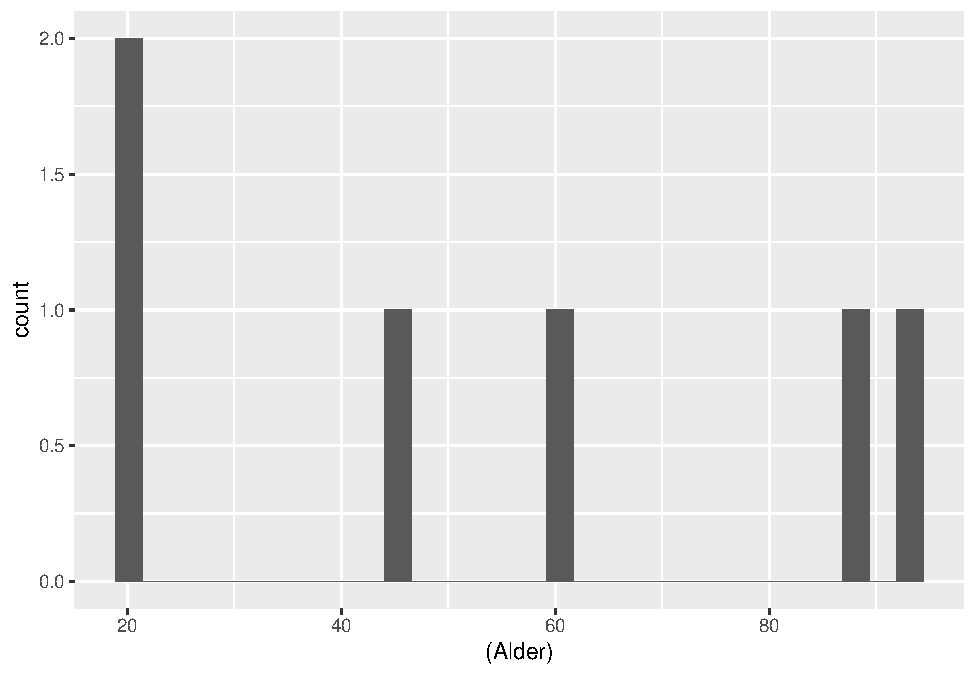
\includegraphics{Seminar_1_files/figure-latex/unnamed-chunk-16-1.pdf}

Det var det for denne gang! På Canvas kommer det til å ligge noen
oppgaver dere kan jobbe med, og bare send spørsmål om dere har noen!
Gleder meg til neste seminar!

\end{document}
